\subsection{Ciclo de carga}

%Carga en dos o tres etapas según la tensión de la batería en el momento de su conexión: precarga, corriente constante y tensión constante. 
Está dividido en dos o tres etapas según la tensión de la batería en el momento de su conexión: precarga, corriente constante y tensión constante \cite{icr18650s3}\cite{ncr18650ga}.

La etapa de precarga sólo tiene lugar en baterías que han sido profundamente descargadas y cuya tensión sea superior a 22V e inferior a 30V.
Se le entrega una corriente constante, cuyo valor se limita a un quinto de la corriente de carga nominal.

Una vez que la batería supera la tensión de 30V, la carga continúa con la etapa de corriente constante hasta llegar a una tensión de 42V.
Su intensidad depende del modo seleccionado en un rango discreto: 1A, 1.6A, 2.1A, 3.2A, 4.3A, 5A, 6.7A.

En la etapa final de tensión constante, se mantiene la tensión de salida en 42V mientras la corriente disminuye hasta un décimo de la corriente nominal de carga,
momento en el cual se produce el corte ya que la batería se encuentra completamente cargada. 

\begin{figure}[H]
    \centering
    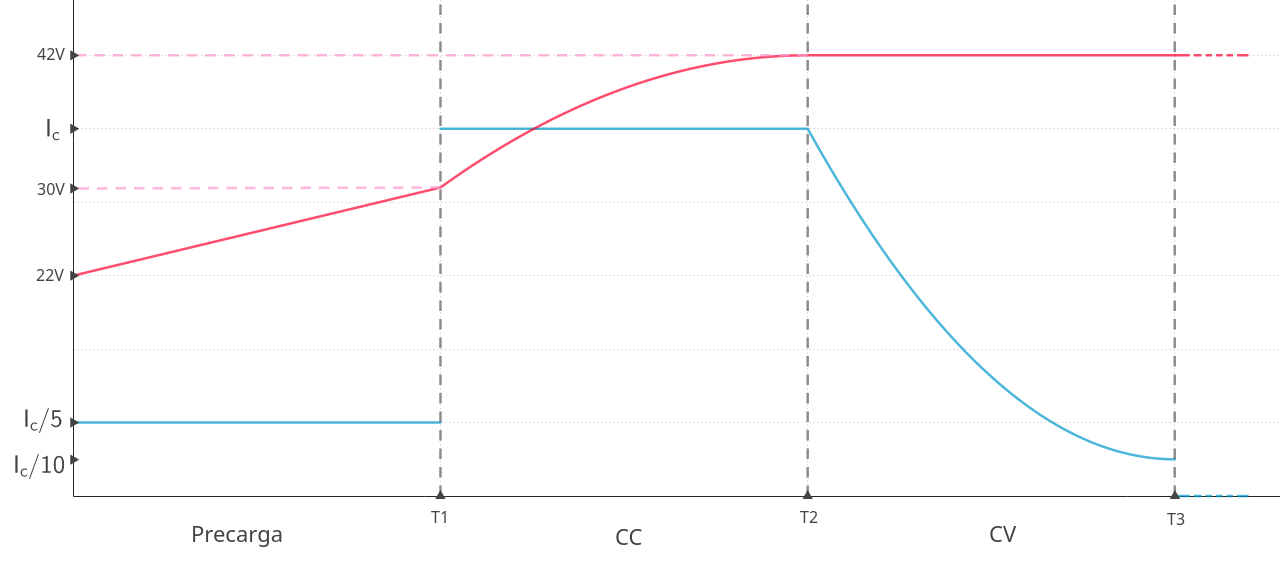
\includegraphics[width=0.8\textwidth]{images/perfil_de_carga.png}
    \caption{Perfil de carga}
    \label{fig:perfil_de_carga}
\end{figure}
